\chapter[Declarative Optimization]{Declarative Optimization}
\label{ch:evita}

Declarative Networking has the potential to expand the lessons and impact of
database technologies into new domains, while reviving interest in classical
database topics like recursive query processing that have received minimal
attention in recent years.  Yet our own system was entirely implemented in an
imperative programming language: the initial version of the P2 runtime was
implemented in C++~\cite{p2:sosp}.  We asked ourselves whether Codd's vision
applies to our own efforts: can declarative programming improve the
implementation of declarative systems?

In this chapter, we put declarative systems ``in the mirror'' by investigating
a declarative implementation of one key component in any relational database
system, the query optimizer.  Specifically, we reimplemented the query
optimizer of P2 as a {\em metacompiler}: a compiler (optimizer) for the P2
language, \OVERLOG, that is itself written in \OVERLOG.  We named the resulting
implementation ``Evita Raced.''\footnote{``Evita Raced'' is almost
``Declarative'' in the mirror, but as with the \OVERLOG language itself, it
makes some compromises on complete declarativity.} Using Evita Raced, we
extended P2 with a number of important query optimization techniques it
formerly lacked, and found that our declarative infrastructure made this quite
elegant and compact.  As we will see in Section~\ref{ch:evita:sec:systemr}, our
implementation of the traditional System R dynamic programming algorithm
comprises only $38$ \OVERLOG rules ($225$ lines of code).  Converting our
System R bottom-up search strategy to a Cascade's style top-down exploration of
the plan space involved minimal effort (less than $24$ hours of programming
time), as we will see in Section~\ref{ch:evita:sec:cascades}.  And our
implementation of the Magic-sets rewriting optimization for recursive queries
in Section~\ref{ch:evita:sec:magic} is not only compact ($68$ rules, $264$
lines), but also nearly a direct translation of the description from Ullman's
course notes on the subject~\cite{ullmanNotes}.

The elegance of our approach was derived in part from the fact that many query
optimization techniques -- like many search algorithms -- are at heart
recursive algorithms, and benefit from a declarative approach in much the same
way as networking protocols.  Even non-recursive optimization logic -- such as
parts of Ullman's magic-sets algorithm -- are simple enough to express in a
declarative fashion that abstracts away mechanistic details such as the
scheduling of data-parallel steps (e.g., scanning all rules in a program in
parallel versus sequentially).

Our contributions in this chapter are three-fold.  First, we presented a declarative
architecture for query optimization that is based on metacompilation, reusing
the query executor in a stylized fashion to serve as the engine beneath the
optimization process.  This resulted in an {\em economy of
mechanism}~\cite{Saltzer75theprotection} not afforded by earlier extensible
optimizers (i.e., EXODUS~\cite{exodus}, Starburst~\cite{phh92},
Volcano~\cite{volcano}, OPT++~\cite{opt++}).  Second, we showed that a variety
of traditional and novel query optimizations are easy to express in a
recursive, declarative language.  Finally, we evaluated the simplicity and
applicability of our design via a full-fledged implementation of an \OVERLOG
query optimizer for P2, which also cross-compiles code that runs on the DSN
wireless sensor network platform~\cite{chu-sensys07}.  Based on our experience,
we believe that declarative metacompilation is a clean, architecturally
parsimonious way to build the next generation of extensible query optimizers
for a wide variety of emerging application domains, where the relevant
optimizations are likely to evolve over time.

The remainder of this chapter is organized as follows.  We begin in
Section~\ref{ch:evita:sec:related} with a look at some prior work in the area
of query optimization, focusing primarily on extensible query optimizers.  We
then turn to the architecture of Evita Raced, starting in
Section~\ref{ch:evita:sec:compile} with a description of the steps to compile
an \OVERLOG program into a relational representation.  Compiling code into data
is necessary in order to then express optimizations and rewrites as queries.  A
program containing queries that reference compiled code is packaged up into a
{\em compilation stage}.  Section~\ref{ch:evita:sec:stages} defines the API of
a compilation stage, and describes how we can dynamically install stages into
the compiler at runtime.  We then present three core declarative compilation
stages (packaged with Evita Raced): the System R dynamic program
(Section~\ref{ch:evita:sec:systemr}), the Magic-sets rewrite
(Section~\ref{ch:evita:sec:magic}), and the localization rewrite
(Section~\ref{ch:evita:sec:localization}) for handling distributed joins in
\OVERLOG~\cite{loo-sigmod06}.  We conclude with a discussion of lessons learned
in Section~\ref{ch:evita:sec:discussion} and a brief summary in
Section~\ref{ch:evita:sec:summary}.


\section{Related Work}
\label{ch:evita:sec:related}

The pioneering work on extensible query optimizer architectures was done in the
EXODUS~\cite{exodus} and Starburst~\cite{lohman,phh92} systems, which provided
custom rule languages for specifying plan transformations.  The EXODUS
optimizer generator used a forward-chaining production rule language to iteratively
transform existing query plans into new ones.  Follow-on work
(Volcano~\cite{volcano} and Cascades~\cite{cascades}) exposed more interfaces
to make the search in this space of transformations more efficient.  Starburst
had two rule-based optimization stages.  The SQL Query Rewrite stage provided a
production rule execution engine, for ``rules'' that were written imperatively
in C; it included a precedence ordering facility over those rules.  The
cost-based optimizer in Starburst was more declarative, taking a grammar-based
approach to specifying legal plans and subplans.

While all of this work was rule-based and extensible, most of it only exposed
individual plan transformations to extensibility; the actual search algorithms
or transformation orderings of EXODUS, Volcano, Cascades, and the Starburst
cost-based optimizer were confined to procedural code.  By contrast, Evita Raced
does not embed a search algorithm, instead leaving that open to specification
as needed.  As we show in Section~\ref{ch:evita:sec:systemr}, both the dynamic programming
bottom-up strategy and the Cascades top-down strategy naturally fit to a
Datalog-based rule language.

Another interesting extensible query optimizer is Opt++~\cite{kabradewitt},
which exploits the object-oriented features of C++ to make an optimizer
framework that was easy to customize in a number of ways.  A specific goal of
Opt++ was to make the search strategy extensible, enabling not only top-down
vs.  bottom-up state-space enumeration, but also randomized search algorithms.
Evita Raced embraces these additional dimensions of extensibility introduced by
Opt++, but provides them in a higher-level declarative programming framework.

The cyclic dataflow used for stage scheduling in Evita Raced
(Section~\ref{ch:evita:sec:stages}) resembles the continuous query engine of
TelegraphCQ, with our StageScheduler and Demux elements working together to
behave somewhat like the TelegraphCQ {\em eddy} operator~\cite{tcq-cidr}.  This
connection occurred to us long after we developed our design, but in retrospect
the analogy is quite natural: Evita Raced stages are akin to TelegraphCQ's
``installed'' continuous queries, and P2's \OVERLOG queries are akin to data
streaming into TelegraphCQ.

%Our description of \OVERLOG was based on our understanding of the current state
%of the P2 codebase.  Loo et al.~\cite{loo-sigmod06} describe a language for P2
%they call Network Datalog (NDLog), that is roughly a simple sub-language of the
%current state of \OVERLOG.  NDLog is a subset of Datalog with aggregation, and
%hence does not provide delete rules or updates.  Unlike \OVERLOG, NDLog offers
%well-defined global program semantics across the network, but it does so by not
%offering delete or update rules, which are used in many \OVERLOG programs.

\section{Declarative Compilation}
\label{ch:evita:sec:compile}

Evita Raced is a compiler (i.e., query optimizer) for the \OVERLOG
declarative language that supports a runtime-extensible set of program
rewrites and optimizations, which are themselves expressed in \OVERLOG.
This metacompilation approach is achieved by implementing optimization
logic via dataflow programs  (query plans) running over a set of tables.  Two
main challenges must be addressed to make this work.  First, all
compiler state -- including the internal representation of both
declarative \OVERLOG programs and imperative dataflow programs -- needs
to be captured in a relational representation so that it can be
referenced and manipulated from \OVERLOG.  Second, the (extensible) set
of tasks involved in optimization must itself be coordinated via a
single dataflow program that can be executed by the P2 runtime engine.
In this section we describe the implementation of the Evita Raced
framework, including the schema of the compiler state, the basic
structure of the Evita Raced dataflow graph, and the basic dataflow
fragments needed to bootstrap the optimizer.

\begin{figure*}
\ssp
\begin{center}
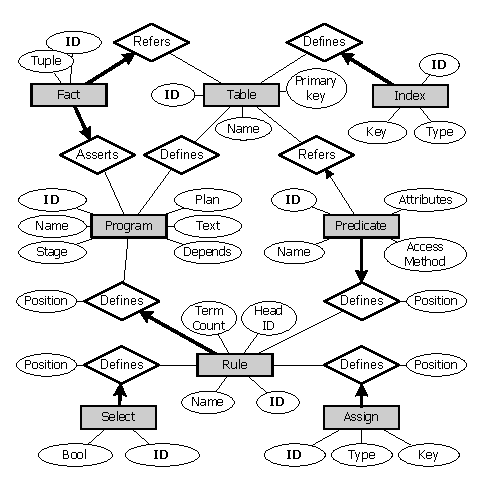
\includegraphics[scale=1.4]{figures/ERDiagram}
\caption{ER Diagram of a query plan in P2. The primary key columns shown in bold.}
\label{ch:evita:fig:p2er}
\end{center}
\end{figure*}

\subsection{Table-izing Optimizer State} 

A typical query optimizer maintains a number of data structures to describe the
contents of a query, and to represent the ongoing state of a query planning
algorithm, including fragments of query plans.  Our first task in designing
Evita Raced was to capture this information in a relational schema.

Figure~\ref{ch:evita:fig:p2er} shows an Entity-Relationship diagram we
developed that captures the properties of an \OVERLOG program, and its
associated P2 dataflow query plans.  We derived the constraints in the diagram
by reviewing the semantic analysis rules enforced in the original P2 compiler;
we discuss a few of them here for illustration.  An \OVERLOG~{\em rule} must
appear in exactly one {\em program}.  A {\em select} term (e.g.,
\ol{f\_contains(X,P2) == false} in Figure~\ref{ch:p2:fig:overlogSP}) is a
Boolean expression over attributes in the predicates of the rule, and must
appear in exactly one {\em rule}.  The diagram indicates that a {\em predicate}
must also appear in a unique {\em rule}, and that it may possibly reference a
single {\em table}.  A predicate that references a table is called a {\em table
predicate} (or a \emph{materialized predicate}), while one that does not
reference a table is called an {\em event predicate}.  An {\em index} is
defined over exactly one {\em table}, and a {\em table} defines at least one
index (namely the primary key index, which P2 always constructs).  Some
relations may contain {\em facts} (input tuples) at startup, each of which must
belong to a single program and must reference a single table.

\begin{figure*}
\ssp
\begin{tabular}{|l|l|p{8cm}|} \hline
{\it Name}& {\it Description} & {\it Relevant attributes} \\ \hline\hline
table     & Table definitions & {\bf table\_id}, primary\_key\\ \hline
index     & Index definitions & {\bf index\_id}, {\bf table\_id}, keys, type \\ \hline
fact      & Fact definitions  & {\bf program\_id}, {\bf table\_id}, {\bf id}, tuple\\ \hline
program   & User program description     & {\bf program\_id}, name, stage, text, depends, plan \\ \hline
rule      & Rules appearing in a program   & {\bf program\_id}, {\bf rule\_id}, name,  term\_count, head\_id \\ \hline
predicate & Relational predicates  & {\bf id}, {\bf rule\_id}, table\_id, name, position, access\_method \\ \hline
select    & Selection predicates  & {\bf id}, {\bf rule\_id}, boolean, position \\  \hline
assign    & Variable substitution statements & {\bf id}, {\bf rule\_id}, variable, value, position \\ \hline 
\end{tabular}
\caption{The Metacompiler Catalog: tables defining an \OVERLOG program and dataflow execution plan.
         The primary key columns are shown in bold. }
\label{tbl:catalog}
\end{figure*}

The conversion from ER diagram to relational format was a textbook
exercise~\cite{DBTextbook}.  Table~\ref{tbl:catalog} lists the set of relations
that capture the entities mentioned in the ER diagram; we refer to this as the
{\em Metacompiler Catalog}.  We modified P2 to create these tables at system
startup, and they are accessible to any \OVERLOG programs (e.g., optimizations)
added to the system.
% In addition, there are compiler constraints that cannot be captured by key
% constraints alone.  For instance, a rule must contain exactly one head and
% one event predicate.  Such checks can be performed by integrity constraints
% written into the compiler logic (possibly as \OVERLOG programs).

\subsection{Metacompiler Architecture}
\label{ch:evita:sec:metaarch}
  
\begin{figure*}[htbp]
\centering
\ssp
\begin{tabular}{|p{2.5cm}|l|p{10cm}|} \hline
{\it Stage name}& {\it Language} & {\it Description} \\ \hline\hline
StageScheduler $(Section~\ref{ch:evita:sec:stageschedule})$ & C++ & Coordinates the compilation of stages.\\ \hline
Parser $(Section~\ref{ch:evita:sec:parser})$  & C++ & Bison based parser. Populates Metacompiler Catalog using program AST.\\ \hline
Planner $(Section~\ref{ch:evita:sec:planner})$ & C++ & Generates a dataflow description from the program data contained in the Metacompiler Catalog.\\ \hline
Installer $(Section~\ref{ch:evita:sec:installer})$ & C++  & Instantiates C++ dataflow objects from a dataflow description. \\ \hline
System~R $(Section~\ref{ch:evita:sec:systemr})$ & \OVERLOG  & Performs System R dynamic programming optimization on all rules. \\ \hline
Cascades $(Section~\ref{ch:evita:sec:cascades})$ & \OVERLOG  & Query optimization based on a top-down search strategy. \\  \hline
Magic-sets $(Section~\ref{ch:evita:sec:magic})$  & \OVERLOG & Rewrites rules to include magic predicates, which act as
selection predicates for constants contained in query predicates. \\ \hline
Localization & \OVERLOG   & Rewrites rules containing a distributed joins into a  localized form. \\ \hline
Delta Rewrite & \OVERLOG  & Converts rules based on materialized tables into an ECA form. \\ \hline
Debug print & \OVERLOG & Add special pretty printer predicates, interposed in certain rules. 
The Planner stage translates these printer predicates into dataflow objects that print the tuples
that pass through. \\ \hline
\end{tabular} 
\caption{Primary Evita Raced compiler stages. }
\label{tbl:stages}
\end{figure*}
  

Optimization logic expressed in \OVERLOG is declarative, and Evita Raced
realizes this logic by converting it to a dataflow program to be executed by
the P2 dataflow subsystem, which was described in Section~\ref{ch:p2:sec:p2}.
In this section we describe how Evita Raced represents query optimization
programs as dataflow, and also the way it orchestrates multiple different
optimization programs through the P2 dataflow framework.

An optimizer built using Evita Raced is composed of an extensible number of
{\em stages}, each of which performs some compilation task on the input
program.  Table~\ref{tbl:stages} describes the primary compiler stages packaged
with the Evita Raced framework.  An Evita Raced stage can be written as a
dataflow program of one or more P2 elements in C++, which are then compiled
into the P2 binary; this is how we implement certain base stages required for
bootstrapping, further described in Section~\ref{ch:evita:sec:bootstrap}.  However,
the power of Evita Raced comes from its support for stages written in \OVERLOG,
which, in addition to being compactly expressed in a high-level language, can
be loaded into a running P2 installation at any time.

A stage programmer registers a new stage with Evita Raced by inserting a tuple
into the \ol{program} relation.  This tuple contains an unique identifier
($program\_id$), a name ($name$), a list of stage dependencies ($depends$), and
the program text ($text$).  Because the \ol{program} relation is used to convey
partial compilation results from stage to stage as well, \ol{program} tuples
also contain attributes for the name of the compiler stage currently operating
on the program ($stage$), and the final physical plan ($plan$), though these
attributes are empty when the programmer first creates the tuple.
Section~\ref{ch:evita:sec:stageschedule} describes the $depends$ attribute, and
its use in the installation of new stages.  The $plan$ attribute pertains to
the physical planner stage, which is described in
Section~\ref{ch:evita:sec:planner}.  We next describe the interfaces to an
Evita Raced compiler stage, after which we discuss the way that multiple such
stages are coordinated.

\subsubsection{The Stage API}

At base, an Evita Raced stage can be thought of as a stream query that listens
for a tuple to arrive on an event stream called \ol{<stage>::programEvent},
where \ol{<stage>} is the name of the stage.  The \ol{<stage>::programEvent}
table contains all the attributes mentioned in the \ol{program} table.  When
such a tuple arrives, the queries that make up that stage execute, typically by
modifying catalog tables in some way.  When a stage competes it inserts a new
\ol{program} tuple, containing the name of the stage in the $stage$ attribute,
into the program table.

To represent this behavior in a stage written in \OVERLOG, a relatively simple
template can be followed.  An \OVERLOG stage must have at least one rule body
containing the \ol{<stage>::programEvent} predicate.  This represents the
ability of the stage to react to new programs arriving at the system.  In
addition, the stage must have at least one rule that inserts a \ol{program}
tuple into the \ol{program} table to signal stage completion.

\subsubsection{Stage Scheduling}
\label{ch:evita:sec:stageschedule}

In many cases, optimization stages need to be ordered in a particular way for
compilation to succeed.  For example, a {\em Parser} stage must run before any
other stages, in order to populate the Metacompiler Catalogs.  The {\em
Planner} must follow any stages written in \OVERLOG, since it is responsible
for translating the relational representation of a query into a dataflow
representation.  And finally, the {\em Installer} stage must follow the {\em
Planner}, since it instantiates dataflow specifications as P2 C++ elements, and
installs them into the P2 runtime.  We will see other specific precedence
constraints in Section~\ref{ch:evita:sec:stages}.

A natural way to achieve such an ordering would be to ``wire up'' stages
explicitly so that predecessor stages directly produce
\ol{<stage>::programEvent} tuples for their successors, in an explicit chain of
stages.  However, it is awkward to modify such an explicit dataflow
configuration upon registration of new stages or precedence constraints.
Instead, Evita Raced captures precedence constraints as {\em data} within a
materialized relation called \ol{StageLattice}, which represents an arbitrary
partial order (i.e., an acyclic binary relation) among stages; this partial
order is intended to be a lattice, with the {\em Parser} as the source, and the
dataflow {\em Installer} as the sink.  
 
To achieve the dataflow connections among stages, the built-in {\em
StageScheduler} component (itself a stage) listens for updates to the
\ol{program} table, indicating the arrival of a new \OVERLOG program or the
completion of a compiler stage for an on-going program compilation.  The {\em
StageScheduler} is responsible for shepherding compilation stage execution
according to the \ol{StageLattice}.  Given a \ol{program} update, the
StageScheduler ''joins with`` the \ol{StageLattic} to identify a next stage
that can be invoked, and derives a \ol{<stage>::programEvent} tuple that will
start the given stage; the contents (attributes) of the
\ol{<stage>::programEvent} tuple are the same as those in the updated
\ol{program} tuple.

\begin{figure*}[htbp]
\begin{center}
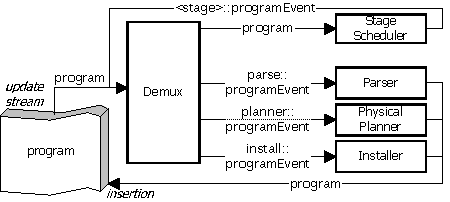
\includegraphics[scale=1.5]{figures/DefaultCompiler}
\ssp
\caption{The Evita Raced (cyclic) dataflow architecture, containing only the default compilation stages.}
\label{ch:evita:fig:basecompiler}
\end{center}
\end{figure*}

The StageScheduler and any compilation stages (whether built-in or
runtime-installed) are interconnected via the simple dataflow illustrated in
Figure~\ref{ch:evita:fig:basecompiler}.  This is the same dataflow architecture
used throughout the {\em Declarative Networking} project.  As described in
Section~\ref{} (and~\cite{p2:sosp}), the dataflow consists of a C++ ``demultiplexer''
that routes tuples from its input (on the left) to individual event handlers
listening for particular tuple names (the arrows leaving the Demux element in
the figure contain the name of the tuple for which the stages to the
right listen).  The Evita Raced framework simply adds the its ''default
stages`` to the bootstrap routine of the P2 system.

Consider the simplicity of how the Evita Raced framework coexists with the P2
dataflow architecture.  To install a new (\OVERLOG) compilation stage into the
runtime, the Installer stage (Section~\ref{ch:evita:sec:installer}) simply extends
the {\em Demux} element to include a port for \ol{<stage>::programEvent}
tuples, routing them to the respective rule(s) of a given stage's \OVERLOG
program. The \ol{StageLattice} relation is also updated (e.g., through fact tuples
in the \OVERLOG stage program) to include its position in the compilation pipeline.
This completes the installation process, after which the \OVERLOG stage need only 
follow a simple protocol for when and how it should execute. 

The protocol to stage execution indicates when it should start (after receiving
a \ol{<stage>::programEvent} tuple) and what it must do on completion.  When a
stage completes, the only requirement is to update the \ol{program} table to
indicate this fact.  The {\em StageScheduler} receives all such updates to the
\ol{program} table -- see Figure~\ref{ch:evita:fig:basecompiler}, the {\em
Demux} \ol{program} tuple port into the {\em StageScheduler} -- and uses the
value of the \ol{program} $depends$ attribute along with the \ol{StageLattice}
relation to determine the next stage.  This completes the full compilation
process in Evita Raced of an \OVERLOG program, from the {\em Parser} stage to the {\em
Installer} stage, and any other stages along the way.

To sum up, the life cycle of a program compilation starts when a user submits a
\ol{program} tuple to the system with a \ol{null} stage attribute.  The
StageScheduler receives that \ol{program} tuple and generates a
\ol{parse::programEvent} tuple (the Parser being the source stage in the
lattice), which is routed by the Demux element to the Parser stage.  When the
Parser is done, it updates that \ol{program} tuple in the corresponding table,
changing the tuple's attribute to ``Parser.'' The StageScheduler receives the
\ol{program} tuple, and routes a \ol{planner::programEvent} to the Demux and
eventually the Physical Planner, which goes round the loop again to the
Installer.  Finally, once the Installer is done and notifies the StageScheduler
via a \ol{program} tuple with the \ol{stage} attribute set to ``Installer,''
the StageScheduler concludes the compilation process.  If the \OVERLOG program
being parsed is itself a new compilation stage, then after installation, the
scheduler updates the stage lattice.


\subsection{Compiler Bootstrapping}
\label{ch:evita:sec:bootstrap}

This section drills down on the stages that make up the baseline Evita Raced
compiler that is now part of P2's bootstrap routine.  As in many
metaprogramming settings, this is done by writing a small bootstrap component
in a lower-level language.  Evita Raced is initialized by a small C++ library
that constructs the cyclic dataflow of Figure~\ref{ch:evita:fig:basecompiler},
including the three default stages shown, which are themselves written in C++.
The entire bootstrap, including the stages is around {\bf 400} lines of C++.
The bootstrap compiler is sufficient to compile simplified \OVERLOG programs
(local rules only, no optimizations) into operational P2 dataflows.  We next
describe each of the three bootstrap stages (Parser, Planner, and Installer) in
a bit more detail, since they form the core foundation of the Evita Raced
framework.

% \jmh{This paragraph was saved from a conflict with Tyson's checkin.  Joe will merge it in Tuesday night.
% The {\em stage scheduler} is a dataflow element that is responsible for providing the inputs to a 
% stage and processing any outputs from a stage. The input to a stage module is a tuple containing the 
% identifier of the program that it is responsible for
% processing. When the stage completes its task is will insert a new program tuple into
% the \ol{program} table with an updated $state$ attribute value that indicates (to the scheduler) the completion 
% of the stage operation on the input program. The program insertion triggers a new
% \ol{programEvent} tuple that is again directed to the stage scheduler, and the process repeats with
% the next scheduled stage in the compilation order. Stage execution order is determined by
% a relation of stage dependencies. The stage scheduler schedules
% a stage based on the dependency graph relation installed by the bootstrap process and the current 
% value of the $state$ attribute in the program tuple. The process completes when the program $state$ 
% attribute reaches stage that no other stage depends on.
% }


% \subsubsection{Default Query Compilation}
% 
% Figure~\ref{ch:evita:fig:basecompiler} shows a dataflow perspective of our default
% metacompiler. A user submits a new program to the system by inserting a tuple into the \ol{program} table.
% The program tuple contains initial values for all the attributes in the program table (see Table~\ref{tbl:tables}). 
% A program table insertion triggers a \ol{programEvent} event tuple that contains the program 
% identifier attribute value.  The "Demux" dataflow element routes the \ol{programEvent} tuple to the
% stage scheduler element, which determines the order in which a stages execute on the input
% program. 
% \petros{The job of the scheduler is a bit nebulous. Is there something
% you can say here to make clear what that does?}
% 
% 
% The input to a stage module is a tuple containing the identifier of the program that it is responsible for
% processing. When the stage completes its task is will insert a new program tuple into
% the \ol{program} table with an updated $State$ attribute value that indicates (to the scheduler) the completion 
% of the stage operation on the input program. The program insertion triggers a new
% \ol{programEvent} tuple that is directed to the stage scheduler, and the process repeats with
% the next scheduled stage in the compilation order. Stage execution order is determined by
% a relation of stage dependencies. The stage scheduler schedules
% a stage based on the dependency graph and the current value of the $State$ attribute in the program tuple. 
% The process completes when the program $State$ attribute reaches stage that no further stage depend on.
% 

\subsubsection{Parser}
\label{ch:evita:sec:parser}

The Parser passes the program text it receives in the \ol{programEvent}
through a traditional lexer/parser library specified using
flex~\cite{flexUrl} and bison\cite{bisonUrl}; this library code returns
a standard {\em abstract syntax tree} representation of the text.
Assuming the Parser does not raise an exception due to a syntax error,
it walks the abstract syntax tree, generating Metacompiler Catalog
tuples for each of the semantic elements of the tree. In addition to
recognizing the different terms of each rule, the parser also annotates
each term with its position in the given program.  By convention, the
first term of a rule body is the event predicate of the rule, if one
exists.  By the same convention, the term in the last position for a
rule is the head predicate.



\subsubsection{Physical Planner}
\label{ch:evita:sec:planner}

The Physical Planner stage is responsible for doing a na\"{i}ve translation of
Metacompiler Catalog tuples (i.e., a parsed \OVERLOG program) into a dataflow
program.  It essentially takes each rule and deterministically translates it
into a dataflow graph language, based on the positions of terms in the rule.

More specifically, for each rule the Planner considers each term (predicate,
selection or assignment) in order of position attribute.  The predicate
representing the event stream is always planned first, and registers a listener
in the Demux element (recall Figure~\ref{ch:evita:fig:basecompiler}).  The
terms following the event stream are translated, left-to-right, into a C++
dataflow in the same way that the original P2 system did, so we do not address
them further here.

We do mention three specific details.  First, whereas the original P2 system
translated a logical query plan directly to a software dataflow structure in
C++, we have chosen to create an intermediate, textual representation of the
dataflow.  This representation is in a language akin to the Click router's
dataflow language, but we omit its details here.

Second, unlike the original P2 system, we have introduced a number of access
methods for in-memory tables.  Our \ol{predicate} relation contains the access
method as one of the attributes, and we have modified the P2 physical planner
to choose the appropriate dataflow element that implements the given access
method.

%% Those are naturally introduced to the P2 physical planner
%% machinery and otherwise
%% creates
%% a listening port in the P2 {\em Demux} on the event stream name. The predicates mentioned in the rule that
%% do not represent the event stream represent lookup operations (joins) on the referenced base relation.
%% A join operator is planned for a predicate by taking the input stream and schema and joining 
%% it - using the $access\_method$ given by the \ol{predicate} tuple - with a base relation producing a new tuple 
%% stream with the join schema. 
%% A selection term plans a filter operator that applies the $boolean$ attribute value to the input 
%% stream and passes only tuples that satisfy this expression to the output stream. \jmh{Again the "plans an operators that does X" doesn't mean much to me.}An assignment term 
%% plans a assignment operator that uses the input stream to evaluate the $value$ attribute (in the \ol{Assign}
%% tuple) to an atomic value. If the input stream contains an attribute named by $variable$ 
%% (in the \ol{Assign} tuple) then the value of that attribute is substituted in the input
%% stream, otherwise a new attribute is added to the input schema with the given value 
%% in the output stream. After all rule body terms have been planned, the planner adds a projection operator
%% that projects the output tuple stream onto the head predicate.

% generates a physical plan for each rule in a program. The execution order of a physical plan in 
% P2 is a leaf-to-root path, with the leaf corresponding to the event predicate and the root being the head 
% predicate. All predicates that lie in between the leaf and the root path are joined against the respective 
% base relation according to the access method given by the predicate tuple. 
% \petros{I would go as far as saying that the physical plan you derive is
% expressed in an operator language reminiscent of the Click
% language. Since we concentrate on logical plan manipulations here we
% don't go into details. The important thing to point out is that whatever
% you do is not tied to a particular runtime; one could take this physical
% plan and install it on a different runtime that isn't our dataflow but
% something else.}

% The initial operator is always the event predicate and it determines when the rule should fire. 
% If the rule does not contain an event predicate then a delta rewrite must be preformed on the rule. 
% The delta rewrite converts the original rule into a set of new rules
% that trigger whenever a side affect\petros{``side affect'' should be
%   ``side effect'' everywhere.} 
% occurs on a table predicate mentioned in the original rule. The delta rewrite is presented 
% in~\cite{boonSigmod}, and we fully adopt this rewrite in our metacompiler. The position attribute 
% defined by each predicate tuple determines the position of the corresponding physical operator in 
% the physical plan. Select and assign operators are also planned at the position indicated by the 
% respective table tuple.

Third, the Planner only understands rules that are in the
event-condition-action (ECA) form. An \OVERLOG rule may have no event
predicate (e.g., ``\ol{table1 :- table2, table3.}'').  A {\em delta rewrite}
(from Loo, et al.~\cite{loo-sigmod06}) is used to convert such rules in an ECA
form (E.g., ``\ol{table1 :- delta\_table2, table3.}'' and ``\ol{table1 :-
table2, delta\_table3.}''.) As in~\cite{loo-sigmod06} \ol{delta\_table} denotes
a stream conveying insertions, deletions, or timeout refreshes to tuples of the
table \ol{table}.  We could have chosen to do this directly in the Planner, but
instead we built it as an \OVERLOG stage.  This decision had an
important consequence; we could only use rules that contained an explicit event
predicate.  Furthermore, any \OVERLOG stage that contained rules with no
explicit event predicate depended on this compilation stage.  The delta rewrite
\OVERLOG stage consists of a mere $6$ rules ($25$ lines of code), and is
usually the first \OVERLOG stage to be compiled into the runtime.
 

\subsubsection{Plan Installer}
\label{ch:evita:sec:installer}

Given the output of the Physical Planner in the dataflow specification
language, what remains is to parse the
textual representation of the dataflow,  construct the
corresponding C++ elements, and ``wire them up'' accordingly. We have
implemented this 
``physical plan compiler'' in C++, and housed it within the
Installer stage.  Once these elements and their connections are
instantiated, the Plan Installer stage stitches them into the P2
runtime's overall dataflow graph, as described in~\cite{p2:sosp}.
As noted in~\ref{ch:evita:sec:metaarch}, this infrastructure made it easy for us to extend P2 with the ability to modify its dataflow graph at runtime,
a feature not available in the released system. 
% Since our focus here
% is on plan optimization, we omit the engineering
% details of that contribution.
% 


\subsection{Discussion}

The metacompilation approach of Evita Raced led us to naturally design the
system extensibility around issues of data storage and dataflow, rather than
library loading and control flow modifications.  While rule-based systems are
usually intended to be easier to extend than a procedural system, the internal
implementation of Evita Raced is especially elegant, due to our thorough
embrace of the native dataflow infrastructure, which we use both to execute
optimization code, and orchestrate stages via precedence tables and the
StageScheduler cycle.  The result of this design is that even a major addition
to the Evita Raced compiler entails very minimal modification to the runtime
state: only the addition of a pair of dataflow edges to connect up the new
stage, and the insertion of precedence tuples in a single table.  Beyond the
StageScheduler and the three bootstrap stages, no additional extensibility code
was added to P2 to support Evita Raced.

Despite its simplicity, Evita Raced is flexible enough that other researchers
have used it to enhance P2 with support for new languages at both its input and
output.  First, by extending the Parser element and registering some \OVERLOG
rules, Abadi and Loo were able to get P2 to optimize and rewrite programs
written in a new language, which extends \OVERLOG with the ability to attest to
the provenance of data in a manner similar to that of~\cite{abadi-netdb07}.
Second, Chu, et al. were able to use Evita Raced to cross-compile \OVERLOG programs
into dataflow specifications that execute on the DSN platform, a declarative
networking system that runs on wireless sensor nodes~\cite{chu-sensys07}.
% In Section~\ref{ch:evita:sec:dsn} we present results from running Evita Raced
% plans in DSN on Berkeley Mote hardware.


\section{Query Compilation Stages}
\label{ch:evita:sec:stages}

% \jmh{This paragraph is thoroughly redundant with hte previous section and can be chopped.  However, it'd be nice to have some kinda warmup text here.}
% A compilation stage written in the P2 query language is dynamically installed into the compiler 
% at runtime, using the same compilation path taken by any \OVERLOG program. The stage programmer 
% inserts a program tuple containing the text of an \OVERLOG program. The programmer also specifies, 
% in the {\em depends} attribute of the program tuple, a single stage that should execute immediately 
% before the installed stage.  After the insertion into the program table, the stage scheduler receives 
% the \ol{programEvent} tuple, which it uses to access the program tuple. The program is processed
% by the stages that appear in the current dependency graph relation. The stages treat the program 
% no differently than any other program. Once the program has been successfully installed, the stage 
% scheduler will then notice that the $depends$ attribute of the program tuple contains a 
% reference to a preexisting stage. 
% The dependency reference informs the stage scheduler that installed program represents a new stage, and 
% that it should update the dependency relation accordingly. After performing the update to the dependency
% relation, the new stage will be included in the compilation process of future input programs. 

Having described the Evita Raced infrastructure, we now turn to the issue of
specifying query optimizations in \OVERLOG.  In this section we describe three
of the compiler stages we have developed for Evita Raced.
Section~\ref{ch:evita:sec:systemr} discusses a dynamic programming optimizer
stage akin to that of System R.  In Section~\ref{ch:evita:sec:cascades}, we
present an optimization that performs a top-down search strategy, which is
modeled after the Cascades optimizer.  Section~\ref{ch:evita:sec:magic}
describes a stage that performs magic-sets rewrite on recursive \OVERLOG
programs.  Finally, Section~\ref{ch:evita:sec:localization} describes our
reimplementation in Evita Raced of the localization rewrite from Loo et
al.~\cite{loo-sigmod06}.

\subsection{System R Optimization}
\label{ch:evita:sec:systemr}

\begin{figure*}
\ssp
\centering
\begin{boxedminipage}{\linewidth}
  {\bf def} optimizer($Q$)
    \begin{algorithmic}[1]
      	\STATE /* Base case: access methods to relations in Q */
  	\FORALL{base relations $R \in Q$}
		\STATE Find all access methods to $R$ and store in $AM$
		\STATE Include index scans iff there exists sargable predicates 
  	\ENDFOR
	\STATE
  	\FORALL{$p \in AM$}
		\IF{$p$ is the cheapest unordered access method \OR 
		    $p$ is the cheapest access method for some "interesting order"}
			\STATE $plans[1] = plans[1] \bigcup p$ 
		\ENDIF
 	\ENDFOR
	\STATE
	\STATE $bp$ = bestplan($|Q|$) /* Get best plans for query Q */
	\IF{$Q$ contains a GROUP BY or ORDER BY}
	 	\STATE $cp$ = cheapest plan $p \in bp$ w.r.t. relevant interesting order 
		\IF{$cp == null$}
			\STATE $cp$ = cheapest overall plan $p \in bp$ + sort operator
		\ENDIF
		\RETURN $cp$
	\ELSE
	 	\RETURN cheapest overall plan $p \in cp$ /* irrespective of ``interesting orders'' */ 
	\ENDIF
    \end{algorithmic}
  {\bf end} \\
  \\
  {\bf def} bestplan(n)
    \begin{algorithmic}[1]
  	\IF{$plans[n] = \emptyset$}
		\FORALL{$p_1 \in plans[1]$} 
			\STATE $P_{n-1}$ = bestplan(n -1)
			\FORALL{$p_{n-1} \in P_{n - 1}$}
			\STATE /* if $p_1$ and $p_{n-1}$ have non-overlapping query predicates */
				\IF{$p_1 \bigcap p_{n-1} = \emptyset$}
					\STATE $plans[n] = plans[n] \bigcup$ all (left-outer) join methods for $p_1$ and $p_{n-1}$
				\ENDIF
			\ENDFOR
		\ENDFOR
		\STATE
		\FORALL{$p \in plans[n]$}
			\IF{$p$ is not the cheapest unordered plan among its equivalent plans \OR
			    $p$ is not the cheapest ``interesting ordered'' plan among its equivalent plans}
				\STATE delete $p$ from $plans[n]$
			\ENDIF
		\ENDFOR
	\ENDIF
	\RETURN plans[n]
      \end{algorithmic}
    {\bf end}
\end{boxedminipage}
\caption{\label{ch:evita:fig:systemr}System R optimizer algorithm.}
\end{figure*}

The System R optimizer paper by Selinger, et al.  is the canonical textbook
framework for database query optimization~\cite{selinger}.  The paper laid out
for the first time the notion that query optimization can be decomposed into
two basic parts: query plan cost estimation and plan enumeration.  While this
algorithm is traditionally implemented inside the heart of a database system
via a traditional procedural programming language, both of these tasks are
naturally specified in a declarative query language.  To perform cost
estimation, System~R requires data statistics like relation cardinalities and
index selectivities; \OVERLOG is a fitting language to collect these
statistics, especially in a distributed fashion over all relation partitions.

Our focus in this section is on the basic dynamic programming algorithm for the
state-space enumeration at the heart of the System R optimizer.
Figure~\ref{ch:evita:fig:systemr} gives a (simplified) sketch of this
algorithm.  It enumerates query plans for increasingly-large subgoals of the
query optimizer.  It fills in a dynamic programming table (e.g., $plans$ in
Figure~\ref{ch:evita:fig:systemr}) with plans that cover a given number of
(relational algebra) predicates that appear in the query.  The dynamic
programming task is to fill in this table with the lowest-estimated-cost query
plan among all plans producing an {\em equivalent} output relation (i.e., plans
composed of the same terms).  The \ol{bestplan} procedure in
Figure~\ref{ch:evita:fig:systemr} captures the essence of generating and
choosing optimal plans with a given number of predicates.

In the System R optimizer, the {\em principle of optimality} is assumed to hold: the
lowest-cost solution to some plan will be built from the optimal solutions to
subplans.  Thus dynamic programming can proceed in ``bottom-up'' fashion.  In a
given program $P$ to be optimized, each rule's event predicate is the
``outermost,'' streaming relation in a query plan for the rule.  For a given
rule $r \in P$, the optimizer generates plans of size $k$ terms by appending a
single (thus unused) term from the rule body to the optimal plan of size $k-1$
terms, as shown in the first loop of \ol{bestplan} in Figure~\ref{ch:evita:fig:systemr}.
There are many additional details that we have chosen to gloss over in the
pseudocode.  

For instance, avoid combining a k-way plan with a 1-way plan if there is no
join predicate between them, unless all predicates have been used up (i.e.,
postpone Cartesian products).  We handle this in our \OVERLOG rules by ensuring
the cost of such an option is greater than any other option that includes join
predicates.  We now turn to describe the \OVERLOG rules for plan generation and
conclude with the rules for best plan selection.

\subsubsection{Plan Generation}
\label{ch:evita:sec:plangen}

\begin{figure*}
\ssp
\centering
\begin{boxedminipage}{\linewidth}
pg1 {\bf plan}(@A, Pid, Rid, PlanID, SubPlanID, Type, TypeID, \\
\datalogspace \xspace \xspace Plan, Schema, Card, Cost, Pos, AM, Sort) :- \\
\datalogspace {\bf systemr::programEvent}(@A, Pid, \_, \_, \_, \_, \_, \_),\\
\datalogspace {\bf predicate}(@A, PredID, Rid, \_, \_, \_, \_, Schema, Pos, \_, \_),\\
\datalogspace Pos == $1$,\\
\datalogspace PlanID := {\em f\_idgen()}, SubPlanID := $null$,\\
\datalogspace Type := "Predicate", TypeID := PredID,\\
\datalogspace Plan := {\em f\_cons}(PredID, $null$),\\
\datalogspace Card := $1$, Cost := $1$,\\
\datalogspace AM := "STREAM", Sort := $null$.
\end{boxedminipage}
\caption{\label{ch:evita:fig:planseed}Plan seed rule.}
\end{figure*}

Figure~\ref{ch:evita:fig:systemr} presents the System R algorithm for plan
generation in two phases.  The first is generating all access methods for a
given relation mentioned in the query (e.g., in the ``from'' clause).
Subsequent to that, a second phase enumerates all possible join orders and
methods.  Recall in Section ? that P2 converts a rule into an
event-condition-action (ECA) form, where the event predicate represents a
stream of tuples from the table reference.  As a consequence of this dataflow
design, our first phase simply generates a plan that listens for such event
tuples.  Extending this rule to consider access methods would entail adding a
predicate that references all access methods to a given relation.

Figure~\ref{ch:evita:fig:planseed} shows the optimizer rule that creates the
initial plan for each rule from the event predicate.  The \ol{plan} tuple
contains a query plan for a given rule, and the plan's \ol{size} reflects the
number of term identifiers in the $Plan$ attribute (i.e., the number of leaves
in the plan tree).  The optimizer listens on the \ol{programEvent} event stream
in rule \ol{pg1}, which initiates the optimization process.  The
\ol{programEvent} tuple is subsequently joined with the \ol{rule} table along
the $Pid$ (program identifier) attribute to obtain the set of rules defined in
the input program.  The resulting set of rule tuples are each joined with the
\ol{predicate} table along the $Rid$ (rule identifier) attribute.  The result
of this join produces a tuple for each predicate term defined by a given rule.
The predicate term assigned to position~$1$ ($Pos == 1$) is by convention the
event predicate term.  For each event \ol{predicate} tuple in each rule of the
input program, rule \ol{pg1} adds a new plan to the \ol{plan} table.  The
$Plan$ attribute represents the initial plan list, starting with the term
identifier ($PredID$) that identifies streaming predicates.  Plan generation
proceeds by appending term identifiers to this list when constructing new plans
from optimal subplans.

The \OVERLOG optimizer defines a set of plan generation rules that together
perform the induction step of the dynamic program.  Each rule extends a best
plan of $k$ terms with a $(k+1)^{st}$, thus far unused term from the rule body.
If the new term considered is a table predicate, then the new plan
annotated with an appropriate join method, which takes the optimal subplan and
``joins it'' with the predicate table.  The join methods supported by P2
include scanned and index-nested-loop-join, as well as merge-join.  A plan
tuple also carries with it an associated cost, which only considers CPU costs
since all P2 relations reside in memory.  We now turn to the description of the
rules that generate plans for nested-loop-join, index nested-loop-join, and
sort-merge join methods.

\begin{figure*}
\ssp
\centering
\begin{boxedminipage}{\linewidth}
\linenumbers
pg2 {\bf plan}(@A, Pid, Rid, {\em f\_idgen()}, PlanID, "Predicate", PredID, \\
\datalogspace \xspace Plan, Schema, Card, Cost, OuterPos+$1$, JM, $null$) :-\\
\datalogspace {\bf bestPlan}(@A, Pid, Rid, PlanID),\\
\datalogspace {\bf plan}(@A, Pid, Rid, PlanID, \_, \_, \_, OuterPlan, \\
\datalogspace \datalogspace OuterSchema, OuterCard, OuterCost, OuterPos, \_, \_),  \\   
\datalogspace {\bf predicate}(@A, PredID, Rid, \_, \_, Tid, \_, PredSchema, PredPos, \_, \_),\\
\datalogspace {\bf rule}(@A, Rid, Pid, \_, \_, \_, \_, TermCount), \\
\datalogspace $PredPos < TermCount$,\\
\datalogspace {\bf table}(@A, Tid, \_, \_, \_, \_, TCard, \_),\\
\datalogspace {\em f\_contains}(PredID, OuterPlan) == $false$,\\
\datalogspace Card := OuterCard * TCard / $10$,\\
\datalogspace Cost := OuterCost + (OuterCard * TCard),\\
\datalogspace JM := NESTED\_LOOP, \\
\datalogspace Plan := {\em f\_cons}(PredID, OuterPlan), \\
\datalogspace Schema := {\em f\_merge}(OuterSchema, PredSchema).\\
\end{boxedminipage}
\caption{\label{ch:evita:fig:plangen1}nested-loop join method.}
\end{figure*}

Any table predicate appearing in a rule body is given a nested-loop-join plan,
shown by rule~\ol{pg2} in Figure~\ref{ch:evita:fig:plangen1}.  The rule is
triggered on an update to the \ol{bestPlan} relation (described in
Section~\ref{}), which contains the plan identifier ($PlanID$) used to select
the reference plan in the \ol{plan} relation.  Each plan tuple contains a list
of the predicate identifiers that already appear in it.  This list is
referenced by the $OuterPlan$ variable in the \ol{plan} predicate of
rule~\ol{pg2}.

The next step is to extend the \ol{plan} tuple with a ``new'' table predicate,
which is done by joining with the \ol{predicate} relation along the same rule
identifier ($Rid$).  The result of this join operation produces all predicates
mentioned in the rule.  To get only the table predicates we join with the
\ol{table} predicate.  The selection predicate $PredPos < TermCount$ ensures that
we do not consider the rule head predicate (last in the rule's terms by
convention).  The function $f\_contains$ tests for containment of the predicate
in the subplan (outer plan).  The tuples that meet the constraints imposed thus
far represent new table predicates that can be used to extend the optimal plan.
We need only assign annotate the new (projected) plan tuple with a join method
(NESTED\_LOOP), associated cost (based on cardinality estimates), a new
predicate list (see $Plan$ variable), and a new schema (see $Schema$ variable).

\begin{figure*}
\ssp
\centering
\begin{boxedminipage}{\linewidth}
pg3 {\bf plan}(@A, ...) :-\\
\datalogspace {\bf bestPlan}(@A, Pid, Rid, PlanID),\\
\datalogspace {\bf plan}(@A, Pid, Rid, PlanID, \_, \_, \_, OuterPlan, \\
\datalogspace \datalogspace OuterSchema, OuterCard, OuterCost, OuterPos, \_, \_),  \\   
\datalogspace {\bf predicate}(@A, PredID, Rid, \_, \_, Tid, \_, PredSchema, PredPos, \_, \_),\\
\datalogspace {\bf rule}(@A, Rid, Pid, \_, \_, \_, \_, TermCount), \\
\datalogspace $PredPos < TermCount$,\\
\datalogspace {\bf table}(@A, Tid, \_, \_, \_, \_, TCard, \_),\\
\datalogspace {\bf index}(@A, Iid, Tid, Key, Type, Selectivity),\\
\datalogspace {\em f\_contains}(PredID, OuterPlan) == $false$,\\
\datalogspace {\em f\_indexMatch}(OuterSchema, PredSchema, Key),\\
\datalogspace Card   := OuterCard * (Selectivity * TCard),\\
\datalogspace Cost   := OuterCost + Card,\\
\datalogspace AM := {\em f\_cons}(Type, Iid),\\
\datalogspace ...
\end{boxedminipage}
\caption{\label{ch:evita:fig:plangen2}index-nested-loop join method (diff from Figure~\ref{ch:evita:fig:plangen1}).}
\end{figure*}

An index-nested-loop join plan is generated by rule \ol{pg3} in
Figure~\ref{ch:evita:fig:plangen2}.  Like rule~\ol{pg2}, it joins the
\ol{bestPlan}, \ol{plan}, \ol{predicate}, and \ol{table} predicates to
get all table predicates referenced by the target rule.  That result is
subsequently joined with the (additional) \ol{index} predicate, which adds
index information to the result tuples.  The function {\em f\_indexMatch} tests
if the index can be used to perform the join using attributes from the best
plan schema ($OuterSchema$) and attributes from the predicate table
($PredSchema$).  Any tuple results from this plan are assigned cardinality and
cost estimates based on some cost function, which uses the additional index
selectivity information given by the $Selectivity$ \ol{index} predicate
attribute.  We also support range predicates in our index-nested-loop join
plans but do not discuss them in detail as they are quite similar to the
nested-loop cases above.

A merge-join performs a join of a plan with a table predicate mentioned in the
rule body along some sorting attribute.  The tuple set from the outer plan and
the predicate table must be ordered by the sorting attribute.  The output of a
merge-join operation preserves the sorting attribute order.  Therefore, the
\ol{plan} predicate generated by the merge-join rule includes the sorting
attribute in the value of the $Sort$ \ol{plan} predicate.  We note that the
$Sort$ attribute in the \ol{table} plan table identifies the sorting attribute
of the table.  A $null$ valued $Sort$ attribute, in either the outer relation
\ol{plan} predicate or the inner relation \ol{table} predicate, means that the
relation is not known to be ordered, and must be presorted prior to the
merge-join operator.  The cost of a merge-join operator depends on need to
presort either relation.

\subsubsection{Best plan selection}
\label{ch:evita:sec:bestplan}

\begin{figure*}
\ssp
\centering
\begin{boxedminipage}{\linewidth}
bp1 {\bf bestCostPlan}(@A, Pid, Rid, Plan, Sort, {\small \bf a\_min}<Cost>) :- \\
\datalogspace {\bf plan}(@A, Pid, Rid, \_, \_, \_, \_, Plan, \_, \_, Cost, \_, \_, Sort, \_). \\
\\            
bp2 {\bf bestPlan}(@A, Pid, Rid, PlanID, Plan2, Cost) :- \\
\datalogspace {\bf bestCostPlan}(@A, Pid, Rid, Plan1, Sort, Cost), \\
\datalogspace {\bf plan}(@A, Pid, Rid, PlanID, \_, \_, \_, Plan2, \_, \_, Cost, \_, \_, Sort, \_), \\
\datalogspace Sort == $null$.\\
\\
bp3 {\bf interestingOrder}(@A, Pid, Rid, PlanID) :- \\
\datalogspace {\bf plan}(@A, Pid, Rid, PlanID, \_, \_, \_, Plan, \_, \_, Cost, \_, \_, Sort, \_), \\
\datalogspace {\bf rule}(@A, Rid, Pid, \_, \_, \_, \_, TermCount), \\
\datalogspace {\bf predicate}(@A, PredID, Rid, \_, \_, Tid, \_, PredSchema, PredPos, \_, \_),\\
\datalogspace {\bf select}(@A, Sid, Rid, Pred, \_, \_), \\
\datalogspace // participates in a later join OR is a prefix of a grouping attribute \\ 
\datalogspace ({\em f\_contains}(PredID, Plan) ==  $false$ \&\& Pred.contains(Sort)) $||$ \\
\datalogspace (PredPos == TermCount \&\& PredSchema.isGroupingAttribute(Sort)). \\
\\
bp4 {\bf bestPlan}(@A, Pid, Rid, PlanID, Plan2, Cost) :- \\
\datalogspace {\bf bestCostPlan}(@A, Pid, Rid, Plan1, Sort1, Cost), \\
\datalogspace {\bf plan}(@A, Pid, Rid, PlanID, \_, \_, \_, Plan2, \_, \_, Cost, \_, \_, Sort2, \_), \\
\datalogspace {\bf interestingOrder}(@A, Pid, Rid, PlanID), \\
\datalogspace {\em f\_setequals}(Plan1, Plan2), Sort1 == Sort2.\\
\\            
\end{boxedminipage}
\caption{\label{ch:evita:fig:bestplan}Best plan selection.}
\end{figure*}

Figure~\ref{ch:evita:fig:bestplan} shows the rules that select the best plan
from a set of equivalent plans, in terms of the output result set and the
ordering properties of the result set.  The \ol{bestCostPlan} predicate of
rule~\ol{bp1} contains the plan with the minimum cost from the set of
equivalent plans.  This aggregation query groups along the program identifier,
rule identifier, plan list~\footnote{The plan lists are actually sets of
predicate identifiers, which forces the grouping operator to use a set
comparison method to test for equivalence.}, and sort attribute.  The inclusion
of the sort attribute in the group condition {\emph enables} the handling of
what Selinger calls ``interesting orders''~\cite{selinger}, along with optimal
subplans.

The remain rules deal with populating the \ol{bestPlan} table with the optimal
unordered and interestingly ordered plans.  Rule~\ol{bp2} selects the best
unordered plan (no ordering attributes $Sort == null$).  An interesting order
is determined in rule~\ol{bp3} by considering the Sort attribute of a plan with
new join predicates and grouping attributes.  The new join predicates are
simply those table predicates not already mentioned in the plan list.  The
grouping attributes are given by the head predicate (in the last position)
through a special method that returns true iff there is a grouping and the Sort
variable references a prefix of the grouping attributes.  This completes our
consideration of interesting orders, since \OVERLOG does not have a notion of
an "order by" clause.  Rule~\ol{bp4} uses the \ol{interestingOrder} predicate
to choose the optimal plan with the given order.
 
\subsubsection{Improving Selectivity Estimation}

For equality selection predications, our System R rules above support selectivity
estimates using a uniform distribution estimator given by the index. For more precise
estimates and to handle range predicates, we have defined declarative rules that produce
equiwidth histograms ({\em ew-histograms}); additional histogramming rules could be
added analogously. The creation of an ew-histogram is triggered by the installation of a
fact in a metadata table of the ew-histograms defined in the system. The metadata table 
contains the parameters of the histogram (i.e., the table name, the attribute position,
and the number of buckets). For example, the fact
\[
\ol{sys::ewhistogram::metadata}(@LOCALHOST, "pred", 3, 10).
\]
creates a ten bucket equi-width historgram on table \ol{pred} for the attribute in the
third position.

Each fact in the ew-histogram table triggers Evita Raced rules that themselves generate
new rules to create ew-histograms (determining bucket boundaries based on the bucket
count and the min and max values of the attribute), and to maintain bucket counts (performing
a count aggregation over the table attributes, grouped by the bucket boundaries). The compiler
stage that generates ew-histograms in this fashion consists of $23$ rules ($92$ lines). The 
histogram data is stored in relational format with each row corresponding to a single bucket.
To exploit these histograms, the cost and selectivity estimation in the \ol{plan} generation rules
in Figures~\ref{ch:evita:fig:plangen1} and~\ref{ch:evita:fig:plangen2} are modified to incorporate
a join with the histogram data relation, and based on the bucket boundaries obtain density 
estimations for a given selection predicate.

\subsection{Top-down Optimization}
\label{ch:evita:sec:cascades}

The bottom-up, dynamic programming search strategy described in
Section~\ref{ch:evita:sec:systemr} is a natural fit to a Datalog-based rule
language.  One might think a top-down Cascades-style optimization
strategy~\cite{cascades} would be hard to implement since \OVERLOG, like
Datalog, is evaluated in a bottom-up fashion.  This is partially true.  Since
the System R search strategy conforms to the \OVERLOG evaluation strategy, it
did not require explicit rules for its traversal through the plan space.  That is,
the System R search strategy was implicitly implemented by the \OVERLOG
bottom-up evaluation.  A top-down search strategy, on the other hand, required
extra logic (three rules) to guide the search through the plan space in
a top-down order.  The logic of a top-down search strategy follows a dynamic
programming technique called memoization, which turns out to be just as natural
and intuitive in \OVERLOG, and hence easily implemented in Evita
Raced.  In this section, we describe our implementation of the Cascades
branch-and-bound algorithm in \OVERLOG.
%, consisting of a mere $33$ rules ($204$ lines).

Our description of the Cascades optimizer follows the notation of Shapiro, et.
al~\cite{Shapiro-opt}.  In Cascades, plans are classified into {\em groups},
which is an equivalence class of expressions (predicates) that produce the same
result.  During the optimization, each group (e.g., [ABC]) represents a
container that references all physical plans (e.g., \{[AB] sort-merge-join
[C]\}, \{[B] nested-loop-join [AC]\}, \ldots) that make up the group.  In order
to keep the search space small, a group only references top-level plans through
{\emph multiexpressions}, which are expressions whose operator takes other
groups as input (e.g., multiexpression \{[AB] sort-merge-join [C]\} takes groups [AB] and
[C] as input).  Associated with each group is a {\emph winner's circle}, which
identifies the optimal plan within a given group, and will be the plan chosen
to represent a given group referenced by a multiexpression.  In the discussion
that follows, a when we indicate a {\emph plan} we mean a given multiexpression
within a group.

We now describe the declarative rules for performing our version of the
Cascades top-down optimization.  The rules are divided into three modules, the
search strategy (Figure~\ref{ch:evita:fig:cascades_top_down}), plan generation
(Figure~\ref{ch:evita:fig:cascades_plan}), and winner selection
(Figure~\ref{ch:evita:fig:cascades_winner}) The rules for winner selection and
plan generation may remind the reader of the best plan selection and plan
generation rules in the System R optimization
(Section~\ref{ch:evita:sec:systemr}).  However, the rules for search strategy
are unique to this optimizer, and will be the focus our attention.
We note that the $9$ rules described here form the
heart of the Cascades optimization in P2, consisting of a total $23$ rules
($204$ lines of code).  The rules not discussed here deal with the P2's lack of
support for stratified Datalog.  Our Cascades optimizer is not stratified but
it is modularly stratified~\cite{rossmodular}, and we require that
each module be fully evaluated bottom-up.  A number of imperative hacks were
required to ensure this requirement in P2, which we defer to the comments
contained in the reference code~\cite{p2code}.

\subsubsection{Search strategy}

\begin{figure*}
\ssp
\centering
\begin{boxedminipage}{\linewidth}
cst1 {\bf group}(Group, Schema) :- \\
\datalogspace {\bf branch}(Group, \_, Cursor, Bound), \\
\datalogspace $Cursor != null$,
\datalogspace Group := Cursor.current(), \\
\datalogspace Schema := Group.schema(). \\
\\
cst2 {\bf branch}(Group, 0, Cursor, Bound) :- \\
\datalogspace {\bf group}(Group, Schema), \\
\datalogspace Cursor := Group.cursor(), \\
\datalogspace Bound  := $infinity$. \\
\\
cst3 {\bf branch}(Group, BranchId+1, Cursor, Bound) :- \\
\datalogspace {\bf bestBranchCost}(Group, BranchId, Cost), \\
\datalogspace {\bf branch}(Group, BranchId, Cursor, OldBound), \\
\datalogspace $Cursor != null$, \\
\datalogspace Cursor := Cursor.next(), \\
\datalogspace Bound := $Cost < OldBound$ ? Cost : OldBound. \\
  
\end{boxedminipage}
\caption{\label{ch:evita:fig:cascades_top_down} Cascades top down search strategy rules.}
\end{figure*}

The optimization begins when the root group (e.g., [ABC]) is inserted into the
\ol{group} table.  A \ol{group} tuple contains an object, as its first
attribute, that provides a cursor to the underlining predicates in the group.
The cursor will generating all subgroups of the given group (e.g., cursor for
group [ABC] will generate subgroups [AB], [BC], [AC]~\footnote{The subgroup
cursors will further generate groups [A], [B], and [C].}).  Rule~\ol{cs2} in
Figure~\ref{ch:evita:fig:cascades_top_down} creates a \ol{branch} tuple from
the initial \ol{group} tuple, using the {\emph cursor} method to create an
initial cursor at position $0$.  A branch contains an upper bound (initialized
to infinity) that is used to prune the cost of plans contained within the given
group.  An insertion into the \ol{branch} table triggers rule~\ol{cst1}, which
inserts the ``current'' subgroup referenced by the cursor object, should one
exists (i.e., no cursor exists for groups containing a single predicate).  When
all plans for the current subgroup have been explored, and a winner selected,
rule~\ol{cst3} advances the cursor to the next subgroup.  This process
completes when the group cursor contains no more subgroups, at which point a
winner can be chosen for the group.


\subsubsection{Plan Generation}

\begin{figure*}
\ssp
\centering
\begin{boxedminipage}{\linewidth}
p1 {\bf plan}(PlanId, Group, BranchId, "tablescan", null, null, Card, Cost) :- \\
\datalogspace {\bf branch}(Group, BranchId, Cursor, Bound), \\
\datalogspace {\bf table}(Name, $\ldots$, Size), \\
\datalogspace $Group.size() == 1$, \\
\datalogspace $Group.tablePredicate() == Name$, \\
\datalogspace PlanId := "tablescan" + Group.id(), \\
\datalogspace Card := Size, \\
\datalogspace Cost := Size. \\
\\
p2 {\bf plan}(PlanId, Group, ``nested-loop'', OuterGroup, InnerGroup, Card, Cost) :- \\
\datalogspace {\bf branch}(Group, BranchId, Cursor, Bound), \\
\datalogspace {\bf winner}(OuterGroup, OuterPlanId, OuterCard, OuterCost), \\
\datalogspace {\bf winner}(InnerGroup, InnerPlanId, InnerCard, InnerCost), \\
\datalogspace {\bf group}(OuterGroup, OuterSchema), \\
\datalogspace {\bf group}(InnerGroup, InnerSchema), \\
\datalogspace $OuterGroup.insersect(InnerGroup) ==  null$, \\
\datalogspace $OuterSchema.joinsWith(InnerSchema) ==  true$, \\
\datalogspace $InnerGroup.size() == 1$, \\
\datalogspace Cost := $OuterSchema.joinsWith(InnerSchema)$ ? \\
\datalogspace \datalogspace OuterCost + (OuterCard * InnerCost) : infinity, \\
\datalogspace $Cost < Bound$, \\
\datalogspace Card := $OuterSchema.joinsWith(InnerSchema)$ ? \\
\datalogspace \datalogspace (OuterCard * InnerCard) / 3 : (OuterCard * InnerCard), \\
\datalogspace PlanId := ``nested-loop'' + Group.id(). \\
\\
p3 {\bf plan}(PlanId, Group, "index-loop", OuterGroup, InnerGroup, Card, Cost) :- \\
\datalogspace {\bf branch}(Group, BranchId, Cursor, Bound), \\
\datalogspace {\bf winner}(OuterGroup, OuterPlanId, OuterCard, OuterCost), \\
\datalogspace {\bf winner}(InnerGroup, InnerPlanId, InnerCard, InnerCost), \\
\datalogspace {\bf group}(OuterGroup, OuterSchema), \\
\datalogspace {\bf group}(InnerGroup, InnerSchema), \\
\datalogspace $OuterGroup.insersect(InnerGroup) ==  null$, \\
\datalogspace $OuterSchema.joinsWith(InnerSchema) ==  true$, \\
\datalogspace $InnerGroup.size() == 1$, \\
\datalogspace {\bf index}(IndexId, Tablename, IndexColumn), \\
\datalogspace $InnerGroup.tablePredicate() == Tablename$, \\
\datalogspace $OuterSchema.join(InnerSchema).contains(IndexColumn) ==  true$, \\
\datalogspace Cost := OuterCost + OuterCard, \\
\datalogspace $Cost < Bound$, \\
\datalogspace Card := (OuterCard * InnerCard) / 3, \\ 
\datalogspace PlanId := "index-loop" + Group.id(). \\
  
\end{boxedminipage}
\caption{\label{ch:evita:fig:cascades_plan} Cascades plan generation rules.}
\end{figure*}

Figure~\ref{ch:evita:fig:cascades_plan} gives three rules for generating plans
in the Cascades optimizer.  The rules are very similar to the plan generation
rules in the System R optimizer (Section{ch:evita:sec:systemr) but are based on
{\emph winner} plans from relevant subgroups.  The schema of the \ol{plan}
table has also changed to reference groups instead of actual plans, as
indicated by the $OuterGroup$ and $InnerGroup$ variables in rules~\ol{p2} and
\ol{p3}.

The plan generation rules are evaluated in a bottom-up fashion by deducing new
plans for a given group.  The \ol{branch} tuple for a given group triggers
each rule.  If the group contains a single table predicate ($Group.size == 1$
in rule~\ol{p1}) then a {\emph table scan} access method is deduced with a cost based
on the number of tuples in the table.  This access method will be selected as
the winner for the single predicate group.  Since P2 only has a table scan
access method we do not consider other access methods (e.g., index).
Additional access methods would include appropriate rules in the form of
Rule~\ol{p1}.

Rules~\ol{p2} and \ol{p3} consider joins of two subgroups (an $OuterPlan$ and
$InnerPlan$) for nested-loop and index-loop join methods.  The rules reference
the optimal plan, contained in the \ol{winner} table, for each subgroup in
order to derive an overall cost for the plan with the given join method.  Each
rule also ensures that the inner plan contains a single table predicate
(left-deep plans only) and that the subgroups do not overlap in the predicates
the consider ($OuterGroup.insersect(InnerGroup) == null$).  We avoid cross
product plans be giving such plans a high cost ($infinity$), which forces such
plans to be considered last.  Since rule~\ol{p3} considers an index-loop join
method, it must check for the existence of an index on the inner predicate that
matches the join attribute.

\subsubsection{Winner Selection}

\begin{figure*}
\ssp
\centering
\begin{boxedminipage}{\linewidth}
wc1 {\bf winner}(Group, PlanId, Schema, Cost) :- \\
\datalogspace {\bf bestCost}(Group, Cost), \\
\datalogspace {\bf branch}(Group, \_, Cursor, \_), \\
\datalogspace $Cursor ==  null$,
\datalogspace {\bf group}(Group, Schema), \\
\datalogspace {\bf plan}(PlanId, Group, \_, \_, \_, \_, \_, Cost). \\
\\
wc2 {\bf bestCost}(Group, {\bf min}$<Cost>$) :- \\
\datalogspace {\bf bestBranchCost}(Group, BranchId, Cost). \\
\\
wc3 {\bf bestBranchCost}(Group, BranchId, {\bf min}$<Cost>$) :- \\
\datalogspace {\bf plan}(PlanId, Group, BranchId, Method, \_, \_, \_, Cost). \\
  
\end{boxedminipage}
\caption{\label{ch:evita:fig:cascades_winner} Cascades winner selection rules.}
\end{figure*}

The rules in Figure~\ref{ch:evita:fig:cascades_winner} select a {\emph winner} plan
from the plans deduced for a given group. We begin with rule~\ol{wc3}, which
determines the optimal plan in a given group. The cost of this optimal plan is
used to update the upper bound for the next branch taken by the search strategy.
Rule~\ol{wc2} further aggregates the result of rule~\ol{wc3} to determine the
best overall plan for a given group, which is used to select a winner for the
group in rule~\ol{wc1}. We must ensure however that a winner is only selected when
the group has been fully explored, which occurs after the cursor ($Cursor$) in
the \ol{branch} table for the group takes on a $null$ value. 


\subsubsection{Summary}

With the details of the rules behind us, we summarize the above discussion
here.  The optimizer generates groups in a top-down order and within each group
it performs a bottom-up search for the cheapest plan, called the {\em winner}.
An upper bound is assigned to each group, contained in the \ol{branch} table,
and initialized to $inifinty$, which is updated as new (cheaper) plans for the
given group are discovered.  A plan (and all its subplans) is pruned if its
cost exceeds the group upper bound.  The optimization terminates when a root
group (containing all expressions in the query) has been fully explored and a
winner has been chosen.

%Suppose the initial query is $A \Join B \Join C$.  The optimizer first
%initalizes the \ol{winner} relation with the root group [ABC]. 
%A single
%rule seeds the recursive rule \ol{c1} in Figure~\ref{ch:evita:fig:bb} by
%initializing the \ol{branch} relation with a tuple that defines the root group
%(i.e., $ABC$) and starts the optimization at position $0$ with predicates ($A$,
%$B$, $C$) and a bound of \ol{infinity}.  The recursion proceeds in a top-down
%fashion.  In the first step a new \ol{branch} tuple is generated that removes
%the predicate in position $0$ generating the group $BC$.  Another rule will
%generate a branch group $A$ at the same time.  The recursion returns when a
%winner for group $ABC$ has been discovered, which occurs when groups $A$ and
%$BC$ have been fully explored and the \ol{next} branch position (e.g., $1$) is
%set for group $ABC$.  A group has been fully explored when its branch position
%reaches the end.  As new winners are discovered the \ol{Bound} variable is
%updated with the winning cost before proceeding to the next predicate.

\subsection{Magic-Sets Rewrite}
\label{ch:evita:sec:magic}

Datalog-oriented systems like P2 perform a bottom-up (\emph{forward chaining})
evaluation on each rule, starting with known facts (tuples), and recursively
deriving new facts through rule deductions.  The advantage of this strategy is
that the evaluation is data driven (from known facts to possible deductions)
and will not enter infinite loops for some statically verifiable \emph{safe}
programs.  In contrast, top-down (\emph{backward chaining}) evaluation (e.g.,
in the Prolog language), starts with the query predicates as the top-level
goals, and recursively identifies rules whose head predicates unify with needed
goals, replacing them with the subgoal predicates in the rule body, until all
subgoals are satisfied by known facts or rejected when no further recursion is
possible.  The advantage of a top-down evaluation strategy is that it avoids
resolving goals that are not needed by the posed queries.

\begin{figure*}[!t]
\ssp
\centering
\begin{boxedminipage}{\linewidth}
{\bf link}("localhost:10000", "localhost:10001").\\
{\bf link}("localhost:10001", "localhost:10002").\\
...\\
\\
r1 {\bf path}(@X, Y, P, C) :- \\
\datalogspace {\bf link}(@X, Y, C), P := f\_cons(X, Y). \\
\\
r2 {\bf path}(@X, Y, P, C) :- \\
\datalogspace {\bf link}(@X, Z, C1), path(@Z, Y, P2, C2),\\
\datalogspace f\_contains(X, P2) == false, \\
\datalogspace P := f\_cons(X, P2), C := C1 + C2. \\
\\
Query: path(@LOCALHOST, "localhost:10000", P, C).
\end{boxedminipage}
\caption{\label{ch:evita:fig:querySP}Relevant rules copied from Figure~\ref{ch:p2:fig:overlogSP}.}
\end{figure*}

Consider again a snippet of the shortest path program in
Figure~\ref{ch:evita:fig:querySP}.  The query asks for the shortest path from
all nodes to node ``localhost:10000''.  A straightforward bottom-up evaluation
applies the \ol{link} tuples to rule \ol{r1}, creating the initial {\tt path}
tuples.  Rule \ol{r2} derives all \ol{path} tuples, while any \ol{path} tuples
matching ``localhost:10000'' on their second attribute are returned by the
programmer's query.

The bottom-up evaluation generates some \ol{path} tuples that do not have
``localhost:10000'' in the second attribute and therefore cannot satisfy the
programmer's query.  In contrast, a top-down evaluation begins by unifying the
query predicate with the head predicate of rules \ol{r1} and \ol{r2}.
Therefore, the \ol{path} predicate unification binds the $@X$ attribute to the
current node identifier and the $Y$ attribute to ``localhost:10000'' in both
rules, which is carried over to the predicates in the rule body.  The binding
of $@X$ and $Y$ attributes in rules \ol{r1} and \ol{r2} means that these rules
will only look for tuples of the form
\ol{path}$(LOCALHOST,"localhost:10000",P,C)$ as well as tuples that can help
form such \ol{path} tuples, but nothing else.

The magic-sets rewrite is an optimization that can reduce the amount of
computation in recursive Datalog queries by deriving only those tuples that are
relevant to query predicates posed by a program.  It does this by adding extra
selection predicates to the rules of a program to emulate the goal-oriented
execution of top-down evaluation (this is sometimes called \emph{sideways
information passing} or SIP).  Conceptually, given a rule of the form 
\[ H_p \text{\ol{:-}}\ G_1, G_2, ..., G_k \] where $H_p$ is the head predicate $p$ and
$G_{1,...,k}$ are the goal predicates in the order of appearance in the rule, a
magic-sets algorithm intersperses selection predicates $s_{1,...,k}$ to
generate rule \[ H_p \ \text{\ol{:-}}\ s_1, G_1, s_2, G_2, ..., s_{k}, G_k \]
Facts for these selection predicates are generated according to bindings of
attributes, in the user's query or other rule predicates in the program, to
constant values.  In Evita Raced we created a magic-sets rewrite stage written
in Overlog.  The Overlog rules are based on the description of the magic-sets
algorithm given in Ullman's course notes~\cite{ullmanNotes}, which operates in
three phases: program analysis, program rewrite, and filter population.  A very
brief overview by example follows.

\subsubsection{Magic-sets by example}

\begin{figure*}[!t]
\begin{center}
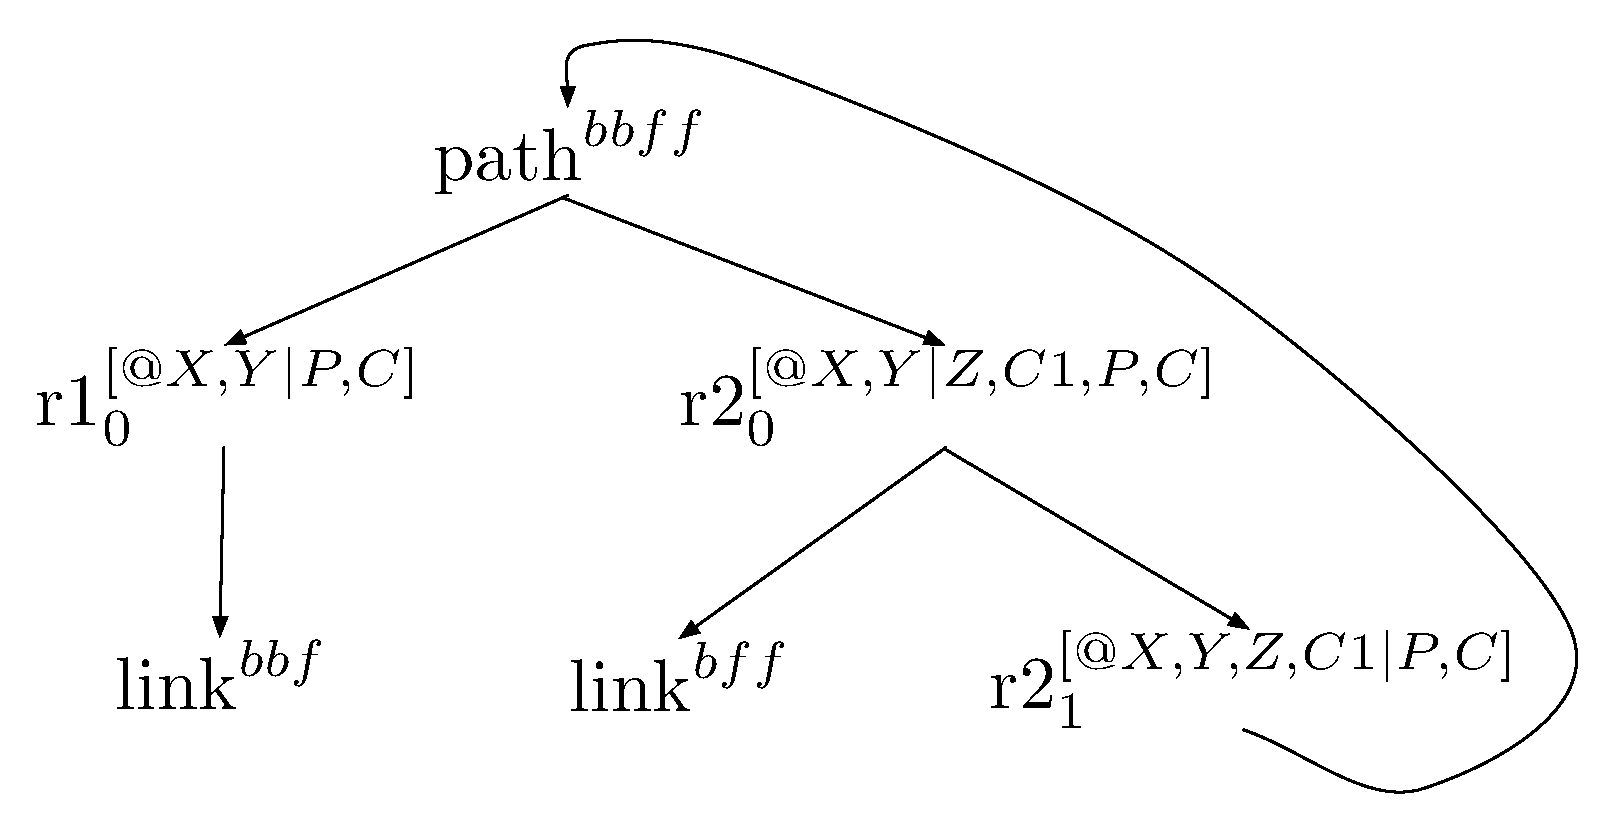
\includegraphics[scale=1.8]{figures/RuleGoalGraph}
\caption{Rule/Goal graph of the program in Figure~\ref{ch:evita:fig:querySP}.}
\label{ch:evita:fig:rggraph}
\end{center}
\end{figure*}

In the program analysis phase, the algorithm considers every rule,
starting with the rule heads that match the query predicate, to build
a recursive tree structure called the {\em Rule/Goal} graph. This graph consists 
of \emph{rule} and \emph{goal} vertices.  A goal vertex consists of a predicate 
with an adornment indicating which of the attributes in the predicate are bound 
to a constant value and which are not bound (free).  A rule vertex represents the bound/free 
state of all seen variables within a rule body, up to a particular position in its left-to-right 
execution. A rule with $k$ body predicates will result in exactly $k$ rule vertices 
corresponding to its positions $[0,...,k-1]$.

Figure~\ref{ch:evita:fig:rggraph} illustrates the full {\em Rule/Goal} graph
for our shortest path example.  To build this graph, the algorithm starts with
a goal predicate (at first, this is the query predicate---\ol{path} in our
example), and creates a goal vertex in the graph with the appropriate adornment
($\mathit{bbff}$ for \ol{path} since the query binds its first two variables to
constant values).  For every rule with that goal predicate as its head, the
algorithm traverses the rule body from left to right, creating a child rule
vertex for every $0$-th position variable binding.  For rule \ol{r2} in the
example, the rule vertex for position $0$ ($r_{2,0}$) has variable state
$[X,Y|P,C]$, which denotes that variables \ol{X,Y} are bound (to the same
values as those ``pushed down'' from the goal vertex) and \ol{P,C} are free.
Given a rule vertex for position $i$, two children are created: a goal vertex
for the next predicate after position $i$ and a rule vertex for the next
position in the rule (unless the body's end has been reached).  In the running
example, the child goal vertex corresponds to the {\tt link} predicate that
appears at position $0$, with adornment $\mathit{bff}$ since \ol{X} is already
bound at this point in the evaluation, but \ol{Z} and \ol{C1} are not.
Similarly, the child rule vertex at position $1$ contains the variable
signature $[X,Y,Z,C1|P,C]$ since \ol{link} added some bound variables.  The
process continues until all rule and goal vertices have been constructed and
connected; only a single goal vertex can exist with the same predicate and
adornment, as is the case for the \ol{path} vertex with adornment
$\mathit{bbff}$.  It is easy to see how the rest of the rule/goal graph is
constructed.  After all vertices have been generated given the chosen rules,
any predicates with a unique adornment in the graph are added to the goals, and
the rules producing them are recursively traversed.


In the program rewrite phase, Ullman's algorithm traverses the rule/goal
graph generating magic predicates for each ``goal'' vertex that is
unique for its (IDB) predicate; in the example, there are multiple vertices
with different adornments for \ol{link}, but only one for \ol{path},
so only \ol{path} is chosen.  This magic predicate is inserted in
the $0$-th position of all rules with the corresponding goal predicate
as the rule head, with the bound variables of the signature as
attributes. In the example, the magic predicate for \ol{path} has the
form \ol{magic\_path(@X, Y)} since \ol{X, Y} are the bound 
variables in the signature of the ``goal'' vertex.  Also
\emph{supplementary} predicates are similarly created for all
encountered ``rule'' vertices during the graph traversal and inserted
within the corresponding original rule.  For example, {\tt sup\_r2\_1(@X,Y,Z,C1)} 
is created for ``rule'' vertex $r_{2,1}$ with the bound variables of
the adornments in the vertex, and placed in the original rule \ol{r2}
between the \ol{link} and \ol{path} predicates.


\begin{figure*}[!t]
\ssp
\begin{boxedminipage}{\linewidth}
{\bf link}("localhost:10000", "localhost:10001").\\
{\bf link}("localhost:10001", "localhost:10002").\\
...\\
{\bf magic\_path}(@LOCALHOST, "localhost:10000"). \\
\\
r1\_g3a {\bf path}(@X, Y, P, C) :- \\
\datalogspace {\bf magic\_path}(@X, Y), \\
\datalogspace {\bf link}(@X, Y, C), P := f\_cons(X, Y).\\
\\
r2\_g1a {\bf magic\_path}(@X, Y) :- \\
\datalogspace {\bf sup\_r2\_1}(@X, Y, Z, C1). \\
\\
r2\_g3a {\bf sup\_r2\_1}(@X, Y, Z, C1) :- \\
\datalogspace {\bf magic\_path}(@X, Y), \\
\datalogspace {\bf link}(@X, Z, C1). \\
\\
r2\_g3c {\bf path}(@X, Y, P, C) :- \\
\datalogspace {\bf sup\_r2\_1}(@X, Y, Z, C1), \\
\datalogspace {\bf path}(@Z, Y, P2, C2). \\
\datalogspace f\_contains(X, P2) == false, \\
\datalogspace P := f\_cons(X, P2), C := C1 + C2. \\
\\
Query: {\bf path}(@LOCALHOST, "localhost:10000", P, C).
\end{boxedminipage}
\caption{\label{ch:evita:fig:magicSP}A magic-sets rewrite of
      the rules in Figure~\ref{ch:evita:fig:querySP} (materialize statements not shown).}
\end{figure*}

Finally, in the filter population phase, the algorithm maintains the
magic predicate relation, which was placed within the rewritten program
in the previous phases.  Any a priori known bindings about the root goal vertex
(e.g., from the user's query) are placed in the magic relation. In the example, the 
fact ``\ol{magic\_path(LOCALHOST, "localhost:10000").}'' is put into the
database from the bindings in the \ol{path} query.  Also, any edges in
the rule/goal graph that start from a rule vertex and end at a goal vertex, with a
unique adornment (i.e., upward arrows in the recursive tree that constitutes the graph), are written as
rules that generate new magic tuples from new tuples of the rule
node's supplementary predicate. In the example, rule \ol{r2\_g1a}~\footnote{Rule names that
deal with magic and supplementary predicate maintenance were named according
to Ullman's rule groups. For instance, rules named \ol{r*\_g3[a-c]} follow rule group 3
and rule \ol{r2\_g1a} follows rule group 1.}  adds
more magic facts as more \ol{sup\_r2\_1} tuples are produced.

Our rewrite implementation of this algorithm first traverses every rule from
head predicate to body predicates from left to right, constructing the
rule/goal graph in the recursive manner of the program analysis, in a single
fixpoint.  Then the new program rules (and replacement of old rules) for the
program rewrite and filter population phases are performed via a traversal of
the newly constructed rule/goal graph in a subsequent fixpoint.  Finally,
initial magic facts are created by direct translation from the query.  Other
details that we elide here involve detecting eligibility of a predicate for a
magic-sets rewrite (whether or not it has a unique adornment in the rule/goal
graph), and state cleanup.

\begin{figure*}
\ssp
\begin{boxedminipage}{\linewidth}
{\bf materialize}(sup,infinity,infinity,keys(2,3,4)). \\
{\bf materialize}(adornment,infinity,infinity,keys(2,5,6)). \\
{\bf materialize}(idbPredicate,infinity,infinity,keys(2,3)). \\
\\
mg1 {\bf goalCount}(@A, Pid, PredName, a\_count$<*>$) :- \\
\datalogspace {\bf idbPredicate}(@A, Pid, PredName), \\
\datalogspace {\bf adornment}(@A, Pid, Rid, Pos, PredName, Sig). \\
\\
mg2 {\bf magicPred}(@A, Pid, GoalName, Sig) :- \\
\datalogspace {\bf goalCount}(@A, Pid, GoalName, Count), \\
\datalogspace {\bf adornment}(@A, Pid, \_, \_, GoalName, Sig). \\
\datalogspace Count == 1. \\
\\
mg3 {\bf sup}(@A, Pid, Rid, Pos, Name, Schema) :- \\
\datalogspace {\bf magicPred}(@A, Pid, Name, Sig), \\
\datalogspace {\bf rule}(@A, Rid, Pid, \_, HeadPid, \_, \_, \_), \\
\datalogspace {\bf predicate}(@A, HeadPid, Rid, \_, Name, \_, \_, Schema, \_, \_, \_), \\
\datalogspace Schema := {\em f\_project}(Sig, Schema), \\
\datalogspace Name := "magic\_" + Name, Pos := 0. \\
\\
mg4 {\bf supNext}(@A, Pid, Rid, Pos+1, Schema) :- \\
\datalogspace {\bf sup}(@A, Pid, Rid, Pos, Name, Schema). \\
\\
mg5 {\bf sup}(@A, Pid, Rid, Pos, Name, Schema) :- \\
\datalogspace {\bf supNext}(@A, Pid, Rid, Pos, PrevSupSchema),\\
\datalogspace {\bf rule}(@A, Rid, Pid, RuleName, \_, \_, \_, \_),\\
\datalogspace {\bf predicate}(@A, \_, Rid, \_, \_, \_, \_, Schema, Pos, \_, \_),\\
\datalogspace Name := "sup\_" + RuleName + "\_" + {\em f\_tostr}(Pos),\\
\datalogspace Schema := {\em f\_merge}(PrevSupSchema, PredSchema).\\
\\
mg6 {\bf adornment}(@A, Pid, Rid, Pos, PredName, Sig) :- \\
\datalogspace {\bf supNext}(@A, Pid, Rid, Pos, PrevSupSchema),\\
\datalogspace {\bf idbPredicate}(@A, Pid, PredName), \\
\datalogspace {\bf rule}(@A, Rid, Pid, \_, \_, \_, \_, \_),\\
\datalogspace {\bf predicate}(@A, \_, Rid, \_, PredName, \_, \_,Schema, Pos, \_, \_),\\ 
\datalogspace Sig := {\em f\_adornment}(PrevSupSchema, Schema).
\end{boxedminipage}
\caption{\label{ch:evita:fig:magicRules}Rule/Goal graph traversal rules.}
\end{figure*}

To give a flavor of the \OVERLOG implementation of Magic Sets,
Figure~\ref{ch:evita:fig:magicRules} shows six rules that build the state
necessary in the magic-sets rewrite by traversing the rule/goal graph.  The
\ol{adornment} predicate contains the predicate name ($PredName$) and an
adornment string ($Sig$), which is initially populated with the query predicate
adornments.  Rule \ol{mg1} counts the number of adornments for each {\em IDB}
predicate.  If this count is unique ($Count == 1$) in rule \ol{mg2}, then a
\ol{magicPred} tuple is created.  Rule \ol{mg3} triggers on a \ol{magicPred}
tuple and, for each rule whose head predicate is named by the \ol{magicPred}
tuple, it generates a \ol{sup} predicate with a $Schema$ attribute containing
the bound variables that exist at the given rule position.  Rule \ol{mg4}
detects a new \ol{sup} predicate (like the one generated for the rule head) and
triggers an event for the subsequent \ol{sup} predicate position in the given
rule.  The three way join in rule \ol{mg5} produces a tuple that contains the
schema of the previous \ol{sup} predicate ($PrevSupSchema$) and the schema of
the predicate ($Schema$) in the subsequent rule position, should one exist.
The head \ol{sup} predicate schema in rule \ol{mg5} contains all the variables
from the previous \ol{sup} predicate and the schema of the current predicate,
since this schema represents the bound variables that will exist in the
subsequent rule position.  Rule \ol{mg6} creates an \ol{adornment} out of the
predicate in the given rule position, if that predicate is part of the {\em
IDB}.  The {\em f\_adornment} function creates a new signature from the bound
variables in the $PrevSupSchema$ attribute, and the variables in the predicate
$Schema$ attribute.  At the end of the rule/goal graph traversal, those
predicates that define a unique adornment are converted into special magic
predicates, and the rules that mention these magic predicates are rewritten
using the information contained in the \ol{sup} table.

\subsubsection{Magic-sets in the Network}

With the details of the magic-sets algorithm behind us, what is
intuitively happening to the shortest-path snippet in
Figure~\ref{ch:evita:fig:magicSP} is that variable bindings in the query are
recursively translated into filtering magic and supplementary
predicates. Since the query is only looking for paths to
destination ``localhost:10000'', at first the magic fact restricts single-hop
paths created from links in rule \ol{r1}) to only those with that same 
destination (in the rewritten rule \ol{r1\_g3a}). Similarly, in what used to 
be rule \ol{r2}, {\tt link} tuples are filtered according to the magic predicate (in rule
\ol{r2\_g3a}), before being joined with existing \ol{path} tuples to
complete the old rule \ol{r2}. The reason rule \ol{r2} was split into
the two rules \ol{r2\_g3a} and \ol{r2\_g3c} is because the
supplementary result \ol{sup\_r2\_1} is useful towards adding extra bindings as
magic tuples (in rule \ol{r2\_g1a}); this is because any variable
binding that survives filtering right before the \ol{path}
predicate in the body of the old rule \ol{r2} is also an interesting
binding for existing or future \ol{path} tuples. If the original
program had not been recursive, then such recursive definitions of magic
facts would not appear in the rewritten program.

\begin{figure*}
\centering

\includegraphics[scale=1.2]{figures/Topology}
\caption{Experimental topology.}
\label{ch:evita:fig:topo}
\end{figure*}

To understand the effects of this rewrite, we describe two experimental
runs of our program, before and after the magic-sets rewrite (both
programs were also subjected to the localization rewrite from
Section~\ref{ch:evita:sec:localization} since they are distributed).  The two
programs are executed in the simple link topology of
Figure~\ref{ch:evita:fig:topo}. Nodes are started up one at a time in order of
identifier, and the preloaded database (EDB) consists of the links pictured. For each experiment we measure the number of
tuples sent and received by each node, as well as any \ol{path}
tuples constructed. The latter measure is meant to convey ``work''
performed by the distributed program even in local computation that does
not appear on the network (e.g., local tuple computations, storage, and
other dependent actions on those tuples).

\begin{figure*}
\centering
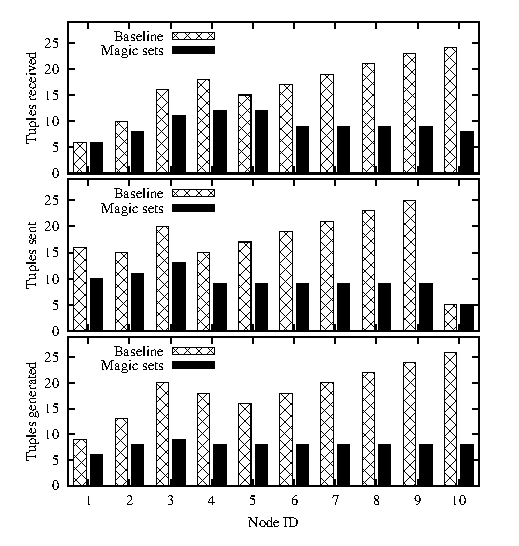
\includegraphics{figures/magicNumbers}
\ssp
\caption{For each node (node ID on $x$ axis), number of tuples received
  (top), sent (middle), and locally generated (bottom) on the $y$ axis.}
\label{ch:evita:fig:magicresults}
\end{figure*}

Figure~\ref{ch:evita:fig:magicresults}(a) shows the number of tuples that each
node receives from the network.  The magic-sets rewritten program causes no
more tuples to be received than the original, and for most nodes significantly
fewer when moving to nodes farther away from the clique.  That is because many
paths that are generated in the original program with destinations within the
clique other than node $1$ are pruned early on and never transmitted all the
way to the far end.  Similarly, Figure~\ref{ch:evita:fig:magicresults}(b) shows
the number of tuples each node transmits.  Again, the magic-rewritten program
does a lot better.  The two programs have similar tuple transmit/receive
overheads for nodes represents the number of tuples a node sends out over the
network.  The inclusion of the magic-sets rewrite reduces the number of sends
in all but one case (node $10$).  The node with identifier $10$ is the only
node with no incoming links and is therefore never burdened with network
traffic other than its own; as a result, though its received tuple overhead
benefits from magic sets, it transmitted tuple overhead is unaffected, since it
already sends out no extraneous paths other than its sole path towards node
$1$.  Finally, tuple storage is impacted beneficially by magic sets everywhere
(Figure~\ref{ch:evita:fig:magicresults}(c)), since both \ol{path} tuples
received from the network, and those generated locally for local consumption
are pruned away by the rewrite.



\subsection{Localization}
\label{ch:evita:sec:localization}

Finally, we briefly describe the localization compiler stage, which turns a
rule with multiple location specifiers in its body to many rules, each of which
has a single location specifier in its body; this essentially turns a
distributed join into a set of local joins with partial result transmissions
among the rules involved~\cite{loo-sigmod06}.  This rewrite was part of the original P2
system, but implemented in C++ and woven into the monolithic compiler.

In Evita Raced, the localization stage traverses distributed rules in
left-to-right order starting with first body predicates (rules with local-only
body predicates are selected out early in the stage).  The location attribute
of the current predicate in this traversal is stored along with the cursor
information of the traversal.  A {\em breakpoint} is generated if the traversal
reaches a predicate with location attribute that differs from the previous.
The breakpoint triggers a {\em split} rule at the given position, which creates
a new {\em glue} predicate $IR_p$, and two new rules defined as follows.
\begin{CompactEnumerate} 
\item $IR_p$ :- (predicates to the left, excluding the breakpoint).  
\item (original rule head predicate) :- $IR_p$, (predicates to the right, including
  the breakpoint).  
\end{CompactEnumerate} 
The location attribute in the $IR_p$ predicate is taken from the predicate at
the breakpoint position.  The other attributes in the $IR_p$ predicate are
taken from the predicates to the left of (and not including) the breakpoint,
which represents the schema of the intermediate result prior to the breakpoint
position predicate.  The algorithm then removes the original rule, and moves
recursively on the second rule, which is considered the original rule in the
above discussion.  The recursion terminates at the rightmost predicate
position.

The localization stage is not an optimization per se, but rather a program
rewrite necessary to make distributed rules executable.
% Any program that contains distributed rules must go through this compilation
% stage.
The \OVERLOG program for localization consists of only 28 rules.  The original
P2 code that performed this task in P2 consisted of approximately 400 lines of
% carefully crafted
C++.

\section{Discussion}
\label{ch:evita:sec:discussion}

When we started this work, the vision of declaratively specified query
optimization was appealing thanks to its elegance and its promise of usability
and maintainability.  Although we remain convinced on this front, our optimism
has been tempered by the pragmatics of developing software within a
continuously changing system prototype.  Here we reflect on some of the (hard)
lessons we learned while conducting this research.

P2's notion of consecutive Datalog-style fixpoints, especially in networked
environments, still has many rough edges, both on the design and on the
engineering front.  Because deep down P2's runtime is an event-driven execution
engine, its basic unit of atomicity is akin to a single iteration through a
recursive query evaluation strategy like semi-naive evaluation, generating a
set of derived actions (tuples to be inserted, deleted, transmitted remotely,
or evaluated locally for further deduction) from a single incoming event, and
committing changes to the database atomically upon completion of such a
step~\cite{LuThesis}.  P2's Datalog-style fixpoints are implemented as
sequences of such single-event iterations, in a manner that appears to have
been an afterthought.  As a result, the system's design shares both
event-driven and logic-style flavors, with some remaining unresolved conflicts,
and no explicit language constructs to bridge between the two.

One example is the notion of \ol{delete} rules, the semantics of which are
unclear.  How is one to handle delete rules triggered by the \emph{deletion} of
a base tuple?  The system certainly does not support -- semantically or
operationally -- the ``undeleting'' of tuples that were originally deleted due
to a base fact that is no longer in the database.  Similarly, the semantics for
multiple updates to the same tuple within the same fixpoint are undefined and a
local tie breaking rule is chosen to decide on a consistent ordering among
same-fixpoint updates to the same relation.  Compiler stages that do static
analysis might catch such dangerous rules and alert the user.

Second, as in most prototypes, the programmer interface is not polished.
Debugging is difficult, especially since the logic language makes it tough to
understand which value corresponds to which formal attribute in a long tuple of
a dozen or more attributes.  Though concise, declaratively specified
optimizations pack a punch in terms of density of concepts, which only becomes
deadlier due to the (otherwise desirable) arbitrary order of rule execution.
Certainly a better thought-out system to debug declarative programs --
optimizations, no less -- would have made the job easier.  To be fair, however,
our experience with building monolithic optimizers in production database
management systems in the past was not a great deal rosier.  It is hard to
debug code when the output's correctness (e.g., minimality of cost) is too
expensive to verify.

Third, the evolution of the \OVERLOG language has a long way to go.  The
language still offers no modularity, making it tough to isolate and reuse
logically distinct components.  It does has a rudimentary concrete type system,
but has poor support for structured types like matrices and lists.  \OVERLOG
still ``cuts corners'' on the proper set-orientation of Datalog; since program
stratification is only preliminary in the system prototype, dealing with
streaming aggregates in the face of EDB updates required us to resort to
imperative tricks like timers and polling to determine that aggregates were
ready to be finalized.

Beyond particular characteristics of P2, one hard lesson we learned was that
extensibility and ease of use at the top often comes at the expense of
complexity below the extensibility layer.  The tabularization of compiler state
to enable declarative optimizations also meant that even imperative compiler
stages such as our bootstrap stages implemented in C++ had to use tables,
foregoing their familiar interaction with C++ data structures.  Building glue
libraries that ease this interaction may relieve this pain.

Nevertheless, despite these complaints, we were able to get all of our desired
optimizations expressed in \OVERLOG in a highly compact way, as promised by the
various earlier papers on P2.  By contrast, the initial version of P2 had no
query optimizations of interest beyond localization.  As \OVERLOG and P2
mature, the use of a metacompilation approach should get even easier.  And
based on our initial experience extending \OVERLOG with security properties in
a manner similar to~\cite{abadi-netdb07}, we believe that our Evita Raced
infrastructure could accelerate the ability of the P2 group to pursue
modifications to \OVERLOG itself.

\section{Summary}
\label{ch:evita:sec:summary}
The Evita Raced metacompilation framework allows \OVERLOG compilation tasks to be written in \OVERLOG and
executed in the P2 runtime engine. It provides significant extensibility via a relatively clean declarative
language. Many of the tasks of query optimization -- dynamic programming, dependency-graph construction
and analysis, statistics gathering -- appear to be well served by a recursive query language. The notion of
metacompilation also leads to a very tight implementation with significant reuse of code needed for
runtime processing.

Even with the caveats expressed in Section~\ref{ch:evita:sec:discussion}, we are convinced that a declarative metacompiler
is much easier to program and extend than the monolithic query optimizers we have worked on previously.
We are now at a  point where we can add significant features (e.g., histograms, broadcast rewrites, 
stratification tests) in an hour or two, where they would otherwise have taken days or weeks of work
in a traditional implementation. 

One surprising lesson of our work was the breadth of utility afforded by the metacompilation framework. Although
motivated by performance optimizations, we have used Evita Raced for a number of unforeseen tasks. These
include: automatically expanding user programs with instrumentation and monitoring logic; generating pretty-printers
for intermediate program forms; language wrappers for secure networking functionality in the manner of
SecLog~\cite{abadi-netdb07}; stratification detectors and other static code analysis. None of these are performance optimizations
per se, but all fit well within an extensible, declarative program manipulation framework. More generally, we believe
that metacompilation is a good design philosophy not only for our work, but for the upcoming generation of
declarative engines being proposed in many fields. 

